\section{Results And Discussion}

\subsection{Metrics}
\noindent
The Mean Per Joint Position Error (MPJPE) is a metric to determine the euclidean distance between the predicted and ground truth 3D poses. This is a common metric used in papers for 3D Pose Estimation \cite{poseestimationreview}. The MPJPE is also computed per keypoint to understand the error distribution. Equation \ref{eq:mpjpe} shows how the euclidean distance error is computed.
\begin{equation}
E = \sum_{i=1} |\mathbf{p_{pred}} (i) - \mathbf{p_{gt}} (i)| \label{eq:mpjpe}
\end{equation}
\noindent
The Percentage of Correct Keypoints (PCK) is a metric to determine if the keypoints are predicted correctly if they fall within the radius of the ground truth keypoints. In this project, PCK@5mm and PCK@15mm are used to evaluate the percentage of correct keypoints if they are 5mm or 15mm within the grouth truth. This metric is easy to understand in terms of measuring accuracy. PCK@5mm is stricter than PCK15mm to measure the precision of keypoints. Equation \ref{eq:pck} shows how the PCK@5mm and PCK@15mm error is computed.
\begin{equation}
Accuracy_{<5/15mm} = \frac{N_{keypoints<5/15mm}}{N_{keypoints}} \times 100\% \label{eq:pck}
\end{equation}

\newpage
\subsection{Hand Pose Evaluation}
\noindent
The models were trained and evaluated using the metrics MPJPE, PCK@5mm and PCK@15mm. Table \ref{table:model_evaluation_hand_pose} shows the performance of the models trained for different architectures - residual blocks, graph convolution layers, and non-local layers. Table \ref{table:model_evaluation_hand_pose} also shows the models trained for different hyperparameters - heat maps, more channels, and fewer channels. Refer to Table \ref{table:model_summary} for exact differences of the model architectures.

\begin{table}[ht]
\centering
\begin{tabular*}{\textwidth}{c @{\extracolsep{\fill}} ccccc}
\hline
Model & Params & FPS & MPJPE & PCK@5mm & PCK@15mm \\
\hline
v1.0 & 13.44M & 12.6 & 8.66 & 30.77 & 87.85 \\ 
v1.1 & 13.30M & 14.77 & 8.24 & 34.68 & 89.04 \\
v1.2 & 16.85M & 13.85 & 8.64 & 32.05 & 87.46 \\
v1.3 & 8.58M & 17.33 & 9.24 & 29.99 & 84.63 \\
v2.0 & 2.08M & 20.16 & 10.61 & 21.73 & 80.08 \\ 
v2.1 & 2.07M & 21.02 & 10.46 & 22.95 & 80.14 \\
v2.2 & 8.20M & 18.14 & 11.84 & 17.24 & 74.90 \\
v2.3 & 0.63M & 22.47 & 12.47 & 17.02 & 70.57 \\
v3.0 & 2.19M & 18.02 & 8.24 & 35.63 & 88.76 \\ 
v3.1 & 2.18M & 19.17 & 8.28 & 33.84 & 89.41 \\
v3.2 & 8.46M & 16.23 & 7.64 & 39.70 & 90.70 \\
v3.3 & 0.72M & 19.40 & 9.10 & 33.65 & 84.90 \\
v4.0 & 2.18M & 18.99 & 8.31 & 34.71 & 88.89 \\ 
v4.1 & 2.17M & 20.00 & 8.63 & 33.26 & 87.76 \\
v4.2 & 8.45M & 17.38 & 8.09 & 37.64 & 88.89 \\
v4.3 & 0.71M & 21.01 & 10.25 & 24.60 & 81.43 \\
[1ex] 
\hline
\end{tabular*}

\caption{Model Evaluation For Hand Pose}
\label{table:model_evaluation_hand_pose}
\end{table}

\noindent
Models v1.X uses 1 convolution layer and 1 residual block for each layer of the 3D Regressor module and generally has low MPJPE error and high PCK accuracy as compared to the other models. However, the number of trainable parameters is almost 7 times more than their counterparts. The residual blocks contributed to most of the paramters. Out of the 4 different hyparameters tested for v1.X, v1.1 that was trained without the heat maps performed the best. v1.2 was trained with more channels but did not show improvements, and v1.3 was traiend with fewer channels and showed worst performance.

\noindent
Models v2.X uses 1 convolution layers for each layer of the 3D Regressor module and did not perform as well as v1.X. The residual block added complexity to the model and allowed it to learn and estimate the 3D poses better. Similar to v1.1, v2.1 also demonstrates the heat maps did not contribute to any improvement in the model performance. v2.2 and v2.3 also similarly show more and fewer channels did not improve the model performance.

\noindent
Models 3.X uses graph convolution layers (SemGCN) and non-local layers instead of the fully-connected layer as the final layer in the 3D Regressor module. v3.1 similarly demonstrates the heat maps did not improve the model performance. v3.3 has fewer channels and performed poorly. Interestingly, v3.2 that was trained with more parameters performed the best out of all the models in this table. The graph convolution layers and non-local layers were able to learn better with more features from the convolution layers.

\noindent
Models 4.X uses graph convolution layers (SemGCN), but unlike 3.X, these models do not have the non-local layers. v4.1 similarly demonstrates the heat maps did not improve the model performance. v4.3 has fewer channels and performed poorly. v4.2 does not perform as well as v3.2. This strongly suggests the non-local layers in v3.2 learn the long distance relationship between entities in the graph, contributing to better 3D pose estimations.

\noindent
Using the results of Table \ref{table:model_summary}, it is evident that Model v3.2 performs the best. However, v3.2 has 4 times more parameters than v3.1. v3.1 still performs reasonably well with fewer paramters. Table \ref{table:model_evaluation_fc} shows the second round of hyperparameters tuning for Model v3.1 to push the model performance further. v3.1.0 has the same architecture as v3.1.0 but the v3.1.0 was further trained end-to-end without freezing the encoder-decoder layers. Models v3.1.x were similarly trained end-to-end, after training the 3D Regressor module alone with the encoder layers freezed.

\begin{table}[ht!]
\centering
\begin{tabular*}{\textwidth}{c @{\extracolsep{\fill}} ccccc}
\hline
Model & Params & FPS & MPJPE & PCK@5mm & PCK@15mm \\
\hline
v3.1.0 & 2.18M & 19.17 & 7.29 & 40.78 & 92.78 \\
v3.1.1 & 2.11M & 20.05 & 7.32 & 41.59 & 92.49 \\
v3.1.2 & 2.24M & 18.38 & 6.93 & 44.52 & 93.64 \\
v3.1.3 & 1.57M & 19.37 & 6.87 & 44.94 & 93.89 \\
v3.1.4 & 2.18M & 19.13 & 8.52 & 30.43 & 89.30 \\
v3.1.5 & 2.18M & 19.17 & 6.87 & 45.27 & 93.56 \\
[1ex] 
\hline
\end{tabular*}
\caption{Model Evaluation (Variations Of v3.1.X)}
\label{table:model_evaluation_fc}
\end{table}

\noindent
v3.1.0 shows that the model did better after further training end-to-end. v3.1.1 shows the model did not perform as well as v3.1.0 after using 2 graph convolution and non-local layers instead of 4. v3.1.2 showed the model performed better using 6 graph convolution and non-local layers instead of 4, although the number of trainable parameters increased by 0.13M. v3.1.3 added 1 more convolution layer at each layer of the 3D Regressor module where the number of output channels of first convolution is half of the number of output channels second convolution layer. This adds depth to model while reducing the number of parameters. Interestingly, the model was able to perform better. v3.1.4 was trained using two loss functions, mean squared error of the 2D poses and mean squared error of the 3D poses. However, the model does not show improvements. v3.1.5 was trained using two loss functions too, mean squared error of the 3D poses and mean squared error of the 3D bone vector. The bone vector encoder the orientation of two joints to correct the direction of the joint positions. The model showed improvements with a higher PCK@5mm.

\begin{table}[ht!]
\centering
\begin{tabular*}{\textwidth}{c @{\extracolsep{\fill}} cccccc}
\hline
Model & Dataset & Full Params & Pose 3D Module Params & MPJPE \\
\hline
Ours & NTU & 23.05M & 1.57M & \(6.79^{*}\) \\ 
L. Ge \cite{handgcn} & NTU & 21.77M & 9.19M & 8.03 \\
Ours & Freihand & 23.05M & 1.57M & \(9.08^{*}\) \\ 
K. Lin \cite{meshgraphormer} & Freihand & 98.43M & - & 6.00 \\
H. Choi \cite{pose2mesh} & Freihand & 74.96M & 67.60M & 7.40 \\ 
[1ex] 
\hline
\end{tabular*}
\caption{Model Evaluation (Benchmark)}
\label{table:model_evaluation_paper_comparison}
\end{table}


\begin{table}[ht!]
\centering
\begin{tabular*}{\textwidth}{c @{\extracolsep{\fill}} cccccc}
\toprule
Model &  \multicolumn{3}{c}{FreiHand} & \multicolumn{3}{c}{NTU} \\[0.5ex] 
\midrule
{} & MPJPE & PCK@5mm & PCK@15mm & MPJPE & PCK@5mm & PCK@15mm \\ 
\hline
Wrist & 9.35 & 18.51 & 88.64 & 6.75 & 44.92 & 96.23 \\ 
Thumb 1 & 8.66 & 20.92 & 91.35 & 5.15 & 64.34 & 97.35 \\
Thumb 2 & 9.56 & 17.25 & 87.43 & 6.10 & 46.15 & 96.80 \\
Thumb 3 & 11.29 & 13.47 & 78.26 & 8.26 & 28.19 & 92.69 \\
Thumb 4 & 16.10 & 6.49 & 58.30 & 10.22 & 20.77 & 86.54 \\ 
Index 1 & 3.88 & 78.09 & 99.37 & 2.65 & 94.91 & 99.23 \\
Index 2 & 6.49 & 42.52 & 96.00 & 6.30 & 55.41 & 93.86 \\
Index 3 & 9.19 & 22.02 & 88.58 & 8.17 & 40.59 & 90.86 \\
Index 4 & 13.64 & 10.08 & 68.89 & 10.76 & 26.61 & 85.36 \\ 
Middle 1 & 1.41 & 100.0 & 100.0 & 1.02 & 99.48 & 100.0 \\
Middle 2 & 5.34 & 54.55 & 98.44 & 5.91 & 56.82 & 95.35 \\
Middle 3 & 9.08 & 21.00 & 89.35 & 7.96 & 39.14 & 91.63 \\
Middle 4 & 14.00 & 8.46 & 68.54 & 10.18 & 26.52 & 86.19 \\ 
Ring 1 & 3.95 & 76.12 & 99.37 & 2.36 & 96.26 & 98.96 \\
Ring 2 & 5.79 & 48.47 & 97.75 & 5.57 & 59.70 & 95.79 \\
Ring 3 & 9.15 & 22.34 & 88.42 & 7.67 & 41.61 & 91.71 \\
Ring 4 & 13.95 & 9.58 & 68.46 & 10.04 & 24.86 & 86.34 \\
Pinky 1 & 6.44 & 39.65 & 97.75 & 4.14 & 78.41 & 98.09 \\
Pinky 2 & 8.12 & 27.25 & 92.72 & 5.96 & 56.47 & 95.30 \\
Pinky 3 & 10.60 & 17.00 & 81.98 & 7.66 & 42.09 & 91.26 \\
Pinky 4 & 14.70 & 8.19 & 64.46 & 9.80 & 29.19 & 85.70 \\
Average & 9.08 & 31.52 & 85.91 & 6.79 & 51.07 & 93.11 \\
[1ex] 
\hline
\end{tabular*}
\caption{Model Evaluation For Keypoints}
\label{table:model_evaluation_keypoints}
\end{table}

\noindent
v3.1.3 shows the model can perform better by adding depth and reducing the trainable parameters. v3.1.5 shows the model can perform better by adding one more loss function. For the final model, the model architecture in v3.1.3 was used and trained using the two loss functions in v3.1.5. The resulting performance is 6.79mm MPJPE on the NTU dataset and 9.08mm MPJPE on the Freihand dataset. Table \ref{table:model_evaluation_paper_comparison} shows our model performance bench-marked against other papers. Note that the asterisk on our model indicates that our model is evaluated differently on the dataset. This is because our model is smaller in size and pose were majority of the joints are occluded are removed from the training and testing dataset. For the NTU dataset, our model does better but it is evaluated without the testing data where majority of the joints are occluded. For the Friehand dataset, our model does not perform as bad as the other state-of-art models. However, note that the number of trainable parameters in the state-of-art models are huge.

\noindent
Table \ref{table:model_evaluation_keypoints} shows the breakdown of the MPJPE, PCK@5mm and PCK@15mm for each joints. The pose centers Middle 1 at the origin and thus the accuracy for this joint is high. It is worth noting that the joints further away from the origin performs worst. Although it is maybe harder to predict the joint position when the joints are further away, the error is also because the joint at the fingers are only connected to 1 neighbouring joint, and the information of that joint is used to estimate its position. The non-local layers might circumvent this issue to some extent, but having more information of more neighbouring nodes might provide better information. Figure \ref{fig:hand_pck_for_different_thresholds} shows the PCK for different threshold on the NTU and Freihand dataset. This table is useful to visualise the precision of the model in estimating the 3D pose.

\begin{figure}[ht]
    \begin{center}
        \begin{subfigure}[b]{0.49\textwidth}
            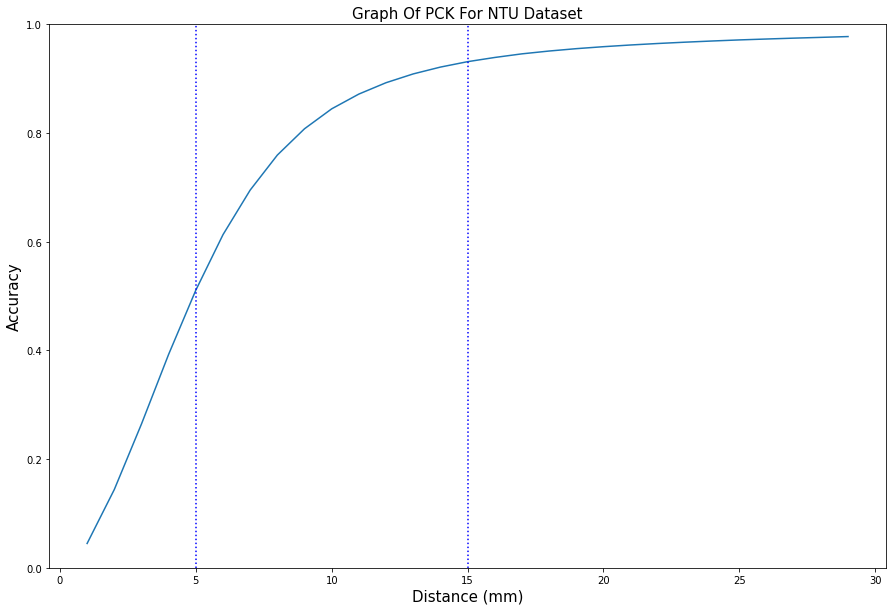
\includegraphics[width=230px]{assets/ntu_pck.png}
            \caption{NTU PCK}
            \label{fig:ntu_pck}
        \end{subfigure}
        \begin{subfigure}[b]{0.49\textwidth}
            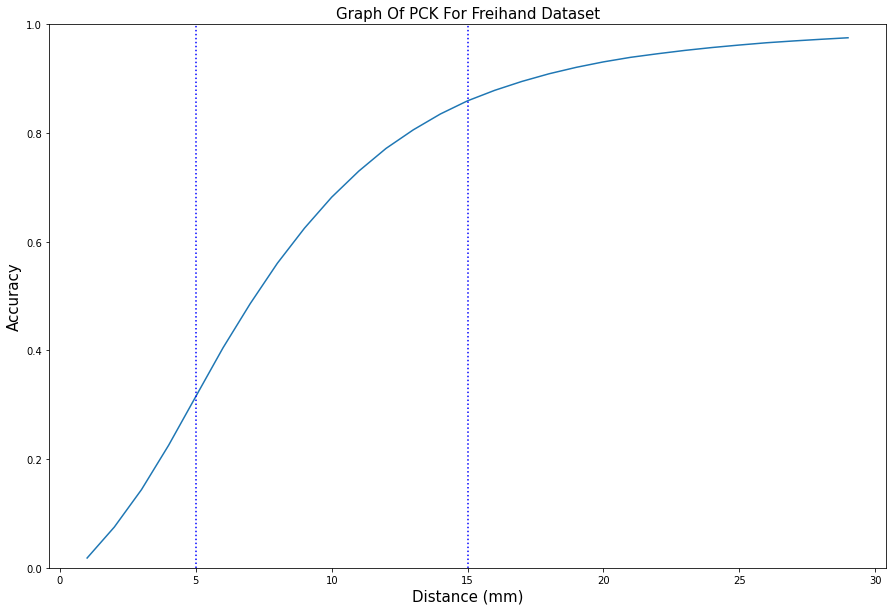
\includegraphics[width=230px]{assets/freihand_pck.png}
            \caption{Freihand PCK}
            \label{fig:freihand_pck}
        \end{subfigure}
	    \caption{Hand PCK For Different Distance Threshold}
	    \label{fig:hand_pck_for_different_thresholds}        
    \end{center}
\end{figure}


\newpage
\subsection{Body Pose Evaluation}
\noindent
Model v3.1.6 is also evaluated on the self-collected dataset for the upper body pose. Table \ref{table:model_evaluation_body_pose} shows the MPJPE, PCK@15mm, and PCK@30mm for each joint and the overall average. This table also compares to performance of v3.1.6 to that of SemGCN where the two 2D poses instead of the image encoded features were used to lift up the 2D poses to 3D.
\begin{table}[ht]
\centering
\begin{tabular*}{\textwidth}{c @{\extracolsep{\fill}} cccccc}
\toprule
Model &  \multicolumn{3}{c}{v3.1.6} & \multicolumn{3}{c}{SemGCN} \\[0.5ex] 
\midrule
{} & MPJPE & PCK@15mm & PCK@30mm & MPJPE & PCK@15mm & PCK@30mm \\ 
\hline
Neck & 8.16 & 94.20 & 100.0 & 24.59 & 42.22 & 77.84 \\ 
Spine & 13.07 & 67.02 & 99.40 & 21.43 & 47.56 & 81.13 \\
LShoulder & 14.13 & 58.02 & 98.56 & 27.72 & 25.58 & 71.29 \\
LElbow & 28.99 & 13.40 & 58.82 & 76.81 & 4.22 & 18.20 \\
LWrist & 37.28 & 9.24 & 40.22 & 93.08 & 3.36 & 16.89 \\ 
RShoulder & 15.16 & 55.73 & 96.38 & 23.49 & 39.00 & 71.13 \\
RElbow & 39.93 & 7.33 & 71.38 & 60.65 & 10.53 & 34.91 \\
RWrist & 50.72 & 7.47 & 29.87 & 80.72 & 1.13 & 9.98 \\
Average & 25.93 & 39.05 & 70.58 & 51.06 & 21.70 & 47.67 \\
[1ex] 
\hline
\end{tabular*}
\caption{Model Evaluation For Body Pose}
\label{table:model_evaluation_body_pose}
\end{table}

\begin{figure}[ht]
    \begin{center}
        \begin{subfigure}[b]{0.49\textwidth}
            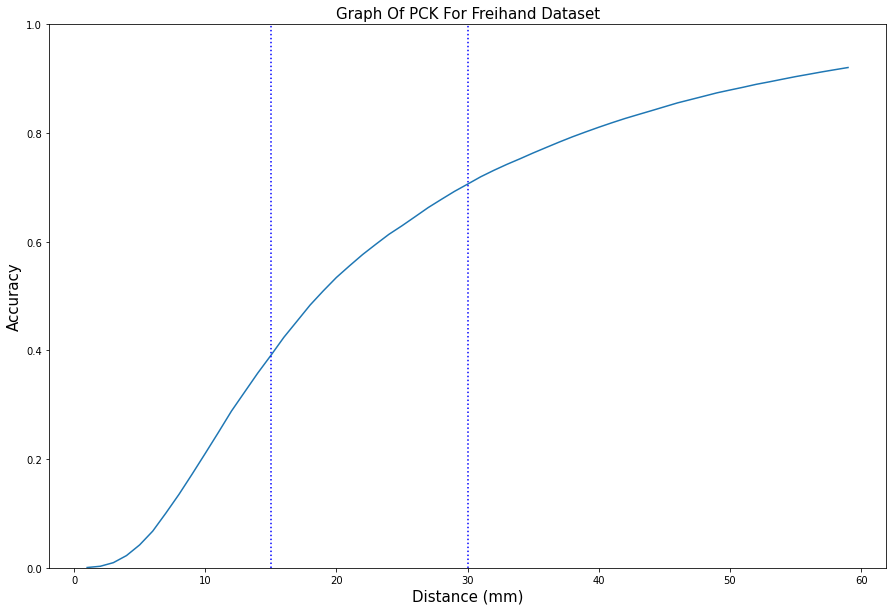
\includegraphics[width=230px]{assets/custom_pck.png}
            \caption{Model v3.1.6 PCK}
            \label{fig:custom_pck}
        \end{subfigure}
        \begin{subfigure}[b]{0.49\textwidth}
            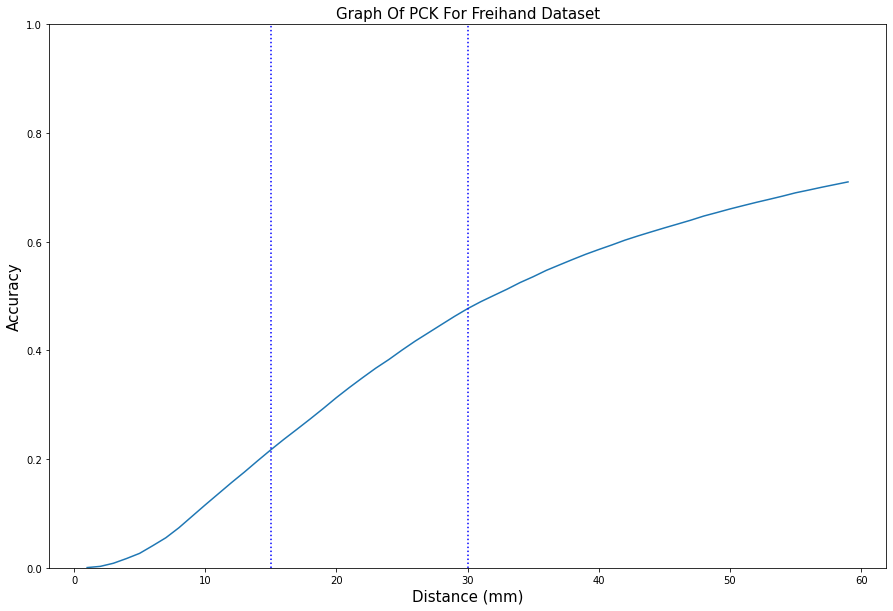
\includegraphics[width=230px]{assets/semgcn_pck.png}
            \caption{SemGCN PCK}
            \label{fig:semgcn_pck}
        \end{subfigure}
	    \caption{Body PCK For Different Distance Threshold}
	    \label{fig:body_pck_for_different_thresholds}        
    \end{center}
\end{figure}

\noindent
The metrics PCK15mm and PCK30mm is used instead of PCK5mm and PCK15mm because the 3D upper body pose covers more distance. Model v3.1.6 performs better than SemGCN because it used the image embeddings to encodes useful features that can help to resolve the ambiguity in the 2D to 3D mapping. However, the performance of v3.1.6 is worst on this upper body pose dataset than the hand pose dataset. This is mainly because the data is collected from the depth camera and cannot precisely measured the joint distance from the camera when it detects the surface of the body. This results in different bone vectors of different magnitude and direction. Figure \ref{fig:body_pck_for_different_thresholds} shows the PCK for different threshold to visualise the precision of the model in estimating the 3D pose.

\newpage
\subsection{Qualitative Results}
\noindent
This section shows Model v3.1.6 inference on the NTU and Freihand testing dataset. Figure \ref{fig:pose_2d_and_3d_on_ntu_hand} shows a sample inference on the NTU dataset that is successful. Figure \ref{fig:pose_2d_and_3d_on_freihand_hand} shows a sample inference on the Freihand dataset that is successful. The inferences shows that the model is able to predict the poses on the testing data relatively well.

\begin{figure}[ht]
    \begin{center}
        \begin{subfigure}[b]{0.32\textwidth}
            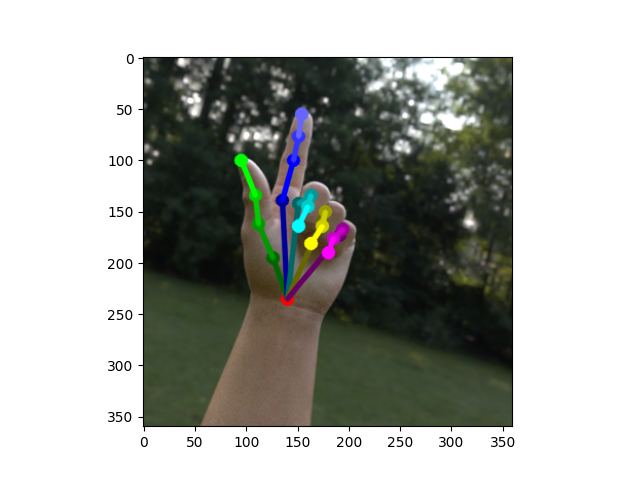
\includegraphics[width=150px]{assets/ntu_2d.png}
            \caption{2D pose}
            \label{fig:ntu_hand_2d}
        \end{subfigure}
        \begin{subfigure}[b]{0.32\textwidth}
            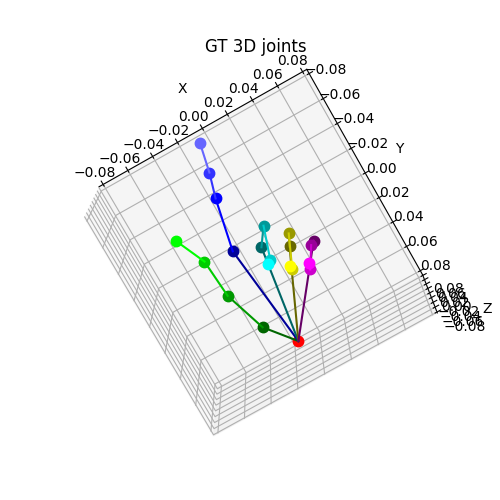
\includegraphics[width=150px]{assets/ntu_3d_gt.png}
            \caption{3D pose}
            \label{fig:ntu_hand_3d_gt}
        \end{subfigure}
        \begin{subfigure}[b]{0.32\textwidth}
            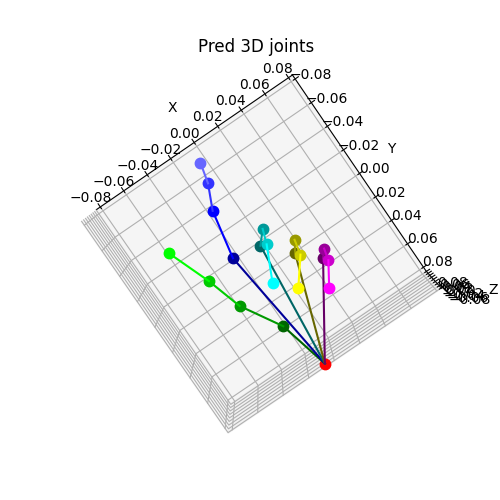
\includegraphics[width=150px]{assets/ntu_3d_pred.png}
            \caption{3D pose}
            \label{fig:ntu_hand_3d_pred}
        \end{subfigure}
	    \caption{Pose 2D and 3D estimation on NTU hand}
	    \label{fig:pose_2d_and_3d_on_ntu_hand}        
    \end{center}
\end{figure}

\begin{figure}[ht]
    \begin{center}
        \begin{subfigure}[b]{0.32\textwidth}
            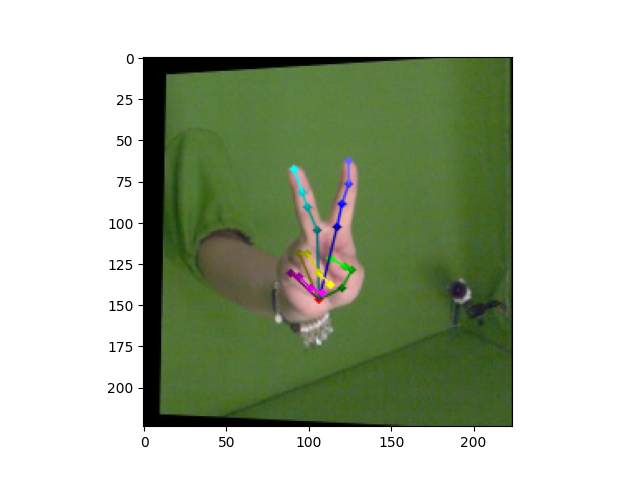
\includegraphics[width=150px]{assets/freihand_2d.png}
            \caption{2D pose}
            \label{fig:freihand_hand_2d}
        \end{subfigure}
        \begin{subfigure}[b]{0.32\textwidth}
            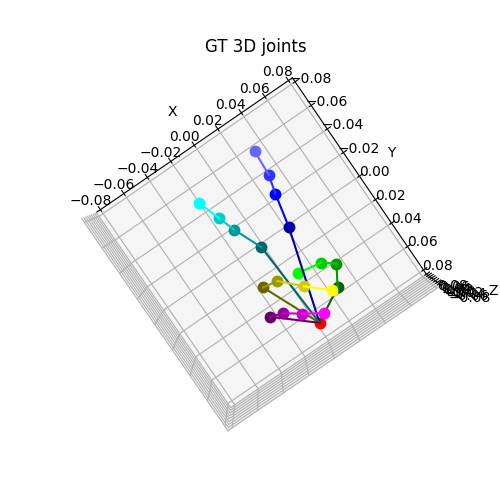
\includegraphics[width=150px]{assets/freihand_3d_gt.png}
            \caption{3D pose}
            \label{fig:freihand_hand_3d_gt}
        \end{subfigure}
        \begin{subfigure}[b]{0.32\textwidth}
            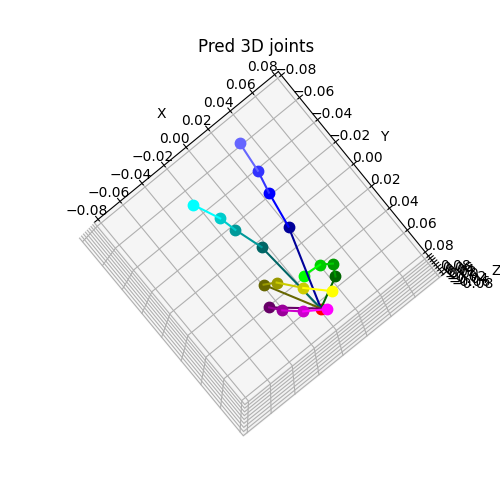
\includegraphics[width=150px]{assets/freihand_3d_pred.png}
            \caption{3D pose}
            \label{fig:freihand_hand_3d_pred}
        \end{subfigure}
	    \caption{Pose 2D and 3D estimation on Freihand hand}
	    \label{fig:pose_2d_and_3d_on_freihand_hand}        
    \end{center}
\end{figure}

\noindent
Figure \ref{fig:pose_2d_and_3d_on_real_hand} shows the pose estimation on a real hand to demonstrate that the model does not perform well on the dataset but can also generalise to other hand as well. The model can also estimate the hand pose when the hand is holding an object. The finger keypoints are important the anchor points to estimate the pose even though the palm keypoints may be occluded.

\begin{figure}[ht]
    \begin{center}
        \begin{subfigure}[b]{0.19\textwidth}
            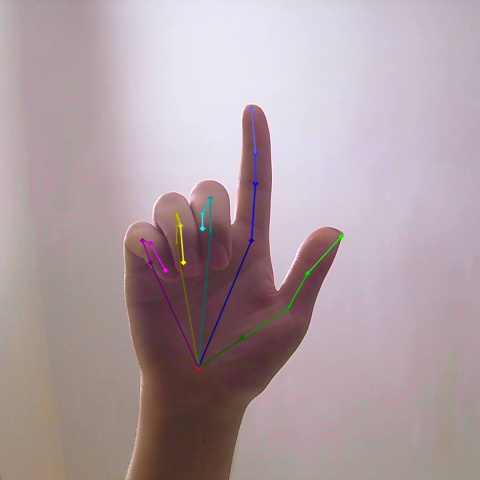
\includegraphics[width=80px]{assets/real_2d.jpg}
            \caption{2D pose}
            \label{fig:real_hand_2d}
        \end{subfigure}
        \begin{subfigure}[b]{0.21\textwidth}
            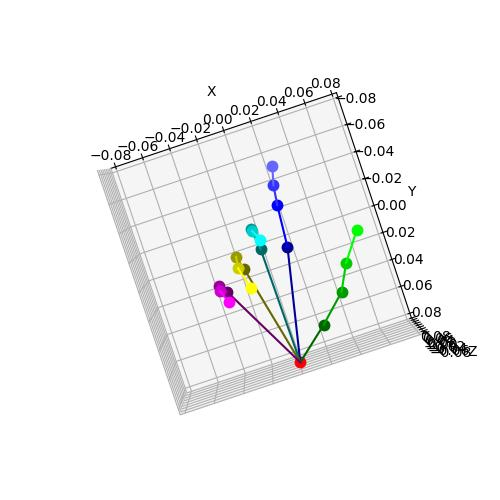
\includegraphics[width=100px]{assets/real_3d.jpg}
            \caption{3D pose}
            \label{fig:real_hand_3d}
        \end{subfigure}
        \begin{subfigure}[b]{0.19\textwidth}
            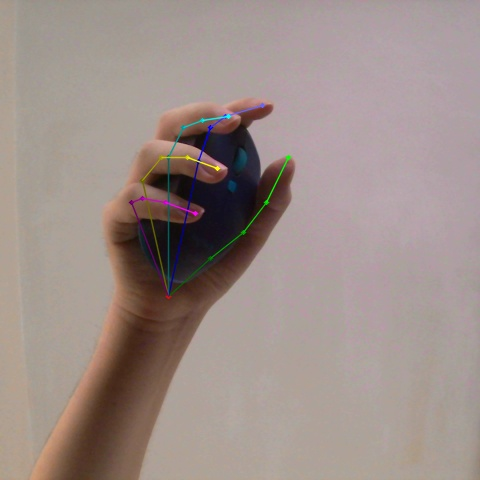
\includegraphics[width=80px]{assets/occluded_2d.jpg}
            \caption{2D Occluded}
            \label{fig:occluded_real_hand_2d}
        \end{subfigure}
        \begin{subfigure}[b]{0.21\textwidth}
            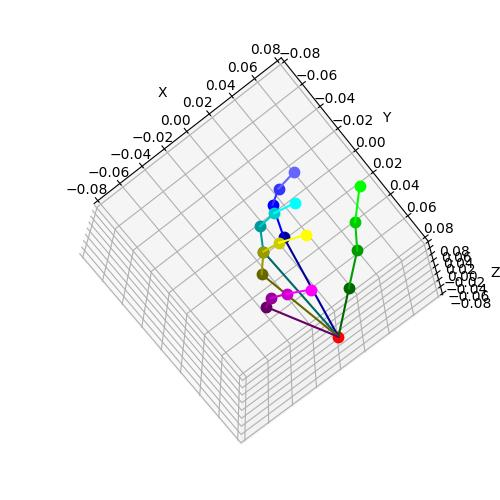
\includegraphics[width=100px]{assets/occluded_3d.jpg}
            \caption{3D Occluded}
            \label{fig:occuluded_real_hand_3d}
        \end{subfigure}
	    \caption{Pose 2D and 3D estimation on real hand}
	    \label{fig:pose_2d_and_3d_on_real_hand}        
    \end{center}
\end{figure}

\noindent
Figure \ref{fig:pose_2d_and_3d_on_failed_hand} shows a failed cased in estimating the 2d pose. However, the estimated 3d pose still has the shape of a hand. The model can give a reasonable estimation of the 3d pose from the encode features of the image. However, SemGCN that lifts the 2d pose to 3d pose cannot give reasonable estimation since the model relies solely on 2d poses.

\begin{figure}[ht]
    \begin{center}
        \begin{subfigure}[b]{0.32\textwidth}
            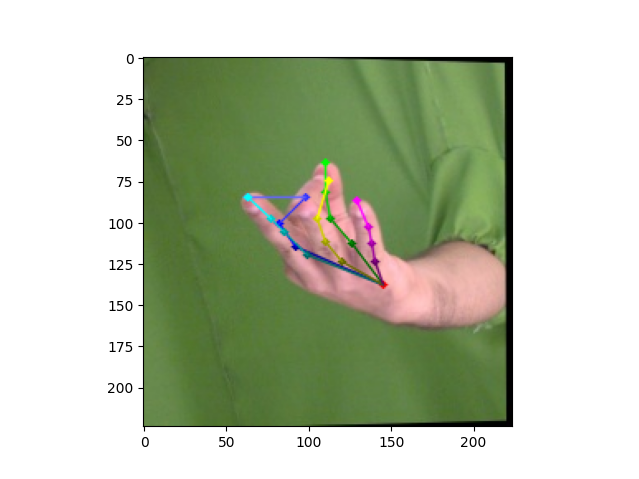
\includegraphics[width=150px]{assets/failed_2d.png}
            \caption{2D pose}
            \label{fig:failed_hand_2d}
        \end{subfigure}
        \begin{subfigure}[b]{0.32\textwidth}
            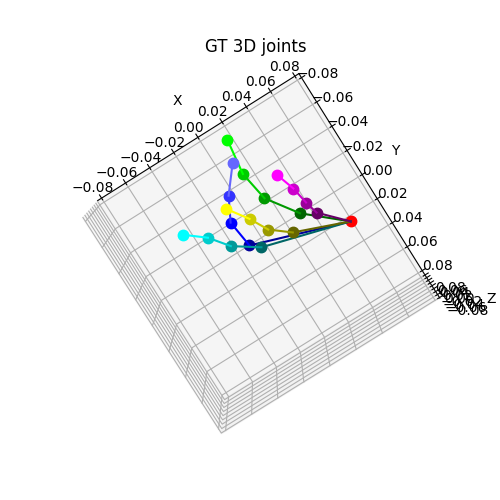
\includegraphics[width=150px]{assets/failed_3d_gt.png}
            \caption{3D pose}
            \label{fig:failed_hand_3d_gt}
        \end{subfigure}
        \begin{subfigure}[b]{0.32\textwidth}
            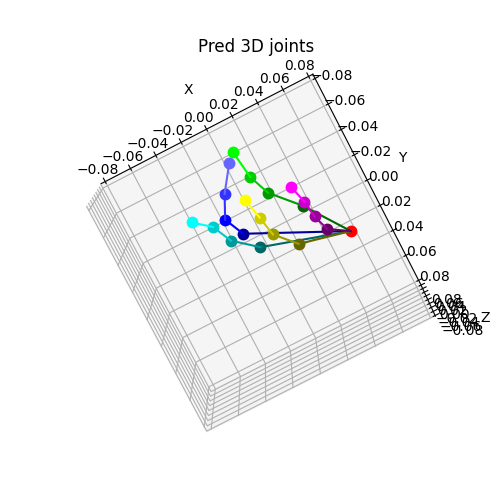
\includegraphics[width=150px]{assets/failed_3d_pred.png}
            \caption{3D pose}
            \label{fig:failed_hand_3d_pred}
        \end{subfigure}
	    \caption{Failed Pose 2D and 3D estimation on Freihand hand}
	    \label{fig:pose_2d_and_3d_on_failed_hand}        
    \end{center}
\end{figure}


\newpage
\subsection{Robotic Arm Teleoperation}
\noindent
After training the pose estimation models, the models were integrated with the robotic arm setup to demonstrate a pick-and-place action. The orientation of the hand is computed from three joints on the palm (Index 1, Pinky 1, and Wrist) to control the orientation of the end effector. The gripper state is computed from the distance between the index tip and the thumb tip (Index 4 and Thumb 4) to open and close the gripper. The position of the end effector is computed from the relative displacement from the initial position of the wrist joint. However, in simulation, it was observed that the position end effector was difficult to control because the upper body pose estimation model was not very precise. Object detection was used instead to track the center of the hand in the image. The displacement of the center of the hand from the center of the image was mapped to the position of the end effector.

\noindent
Figure \ref{fig:pick_and_place_demo} shows the pick and place demonstration in the physical environment. The image on the left is a screen recording that shows the objection detection and pose estimations. It also shows the simulation for testing. The image on the right shows the video recording on the physical robot where the goal is to pick the orange cube and place on the white plate. The cube was picked with the end effector orientated inwards because the robotic arm extends beyond the cube location. The hand shows that the finger and thumb is closed together, corresponding to the closed gripper state. The end effector hovered over the white plate before the cube was released by spreading the thumb and index finger.
\begin{figure}[ht]
	\begin{center}
		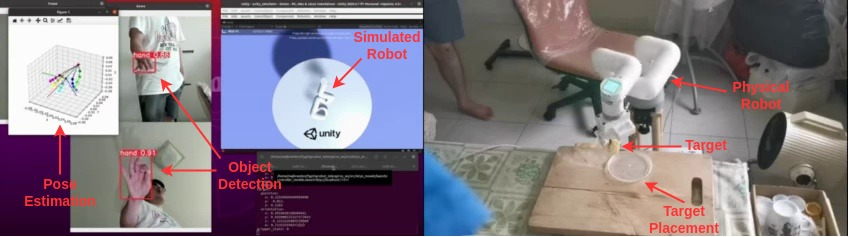
\includegraphics[width=450px]{assets/pick_and_place.jpg}
		\caption{Pick And Place Demonstration}
		\label{fig:pick_and_place_demo}
	\end{center}
\end{figure}